\documentclass[twoside,11pt]{article}

\usepackage{jsat}
\usepackage{amsmath, amsthm, amssymb}
%\usepackage[pdf]{pstricks}
%\usepackage{pst-tree}

%\usepackage[numbers,sort&compress]{natbib}

\usepackage{pifont}
\usepackage{comment}
\usepackage{multirow}
\usepackage{tikz}

\usepackage{listings}
\lstdefinelanguage{smtlib2}
  {alsoletter={-, =},
   morekeywords={set-logic,declare-fun,assert,check-sat,set-info,exit},
   sensitive=false,
   morecomment=[l]{;}}
\lstset{language=smtlib2,
basicstyle=\sffamily,
numbers=none,
keywordstyle=\bfseries\sffamily,
keywordstyle={[2]\bfseries\sffamily\underbar}
}

%\input epsf
\special{papersize=8.5in,11in}

\jsatheading{1}{2004}{25-30}
\ShortHeadings{The SMT Competition 2015--2018}
{Weber et al.}
\firstpageno{25}

\specialcomment{tjark}{\begingroup\footnotesize\color{red}}{\color{black}\endgroup}
\newcommand{\TODO}[0]{\textcolor{red}{TODO}}

\renewcommand{\mark}[0]{\ding{51}}

% TODO
\setcounter{topnumber}{2}
\setcounter{bottomnumber}{2}
\setcounter{totalnumber}{4}
\renewcommand{\topfraction}{0.85}
\renewcommand{\bottomfraction}{0.85}
\renewcommand{\textfraction}{0.15}
\renewcommand{\floatpagefraction}{0.7}

%%%%%%%%%%%%%%%%%%%%%%%%%%%%%%%%%%%%%%%%%%%%%%%%%%%%%%%%%%%%%%%%%%%%%%%%%%%%%%%%

\begin{document}

\title{The SMT Competition 2015--2018}

\author{%
  \name{Tjark Weber (competition chair, 2015--2018)}
  \email{tjark.weber@it.uu.se} \\
  \addr Uppsala University \\
  Uppsala \\
  Sweden
  \AND
  \name{Sylvain Conchon (co-organizer, 2015--2016)}
  \email{Sylvain.Conchon@lri.fr} \\
  \addr Affiliation \\
  City \\
  Country
  \AND
  \name{David D\'{e}harbe (co-organizer, 2015--2016)}
  \email{david@dimap.ufrn.br} \\
  \addr Federal University of Rio Grande do Norte \\
  Natal \\
  Brazil
  \AND
  \name{Matthias Heizmann (co-organizer, 2016--2018)}
  \email{heizmann@informatik.uni-freiburg.de} \\
  \addr Affiliation \\
  City \\
  Country
  \AND
  \name{Aina Niemetz (co-organizer, 2018)}
  \email{niemetz@cs.stanford.edu} \\
  \addr Stanford University\\
  Stanford \\
  USA
  \AND
  \name{Giles Reger (co-organizer, 2017--2018)}
  \email{giles.reger@manchester.ac.uk} \\
  \addr Affiliation \\
  City \\
  Country}

\maketitle

%%%%%%%%%%%%%%%%%%%%%%%%%%%%%%%%%%%%%%%%%%%%%%%%%%%%%%%%%%%%%%%%%%%%%%%%%%%%%%%%

\begin{abstract}
  The International Satisfiability Modulo Theories Competition is an
  annual competition between Satisfiability Modulo Theories~(SMT)
  solvers.  The 2018 edition of the competition was part of the FLoC
  Olympic Games, which comprised 14 competitions in various areas of
  computational logic.  We report on the design and selected results
  of the SMT Competition during the last FLoC Olympiad, from 2015 to
  2018.  These competitions set several new records regarding the
  number of participants, number of benchmarks used, and amount of
  computation performed.
\end{abstract}

\keywords{SMT solver, SMT-COMP, SMT-LIB, Satisfiability Modulo Theories, competitions}

\published{September 2004}{October 2004}{November 2004}

%% Expected content according to the JSAT Call for Papers:

%% Full articles by competition organizers reporting on SAT 2018
%% competitions and evaluation. The articles should describe the
%% competition, its criteria, why it is interesting to the SAT
%% research community, execution environment used, analysis of the
%% results (including how they compare to previous instantiations, if
%% appropriate), and give a summary of the main technical
%% contributions to the field, as well as discussions on lessons
%% learned and suggestions for improvements for future competitions.

%%%%%%%%%%%%%%%%%%%%%%%%%%%%%%%%%%%%%%%%%%%%%%%%%%%%%%%%%%%%%%%%%%%%%%%%%%%%%%%%

\begin{tjark}
Changes 2015:
\begin{itemize}
\item All solvers will be run with $n=4$ cores available.  We will
  recognize both best sequential and best parallel performance in all
  main track divisions, using different CPU time limits.
\item The division scoring will take time spent on unsolved benchmarks
  into account.  Previous competitions only considered time spent on
  solved benchmarks.  However, the number of solved benchmarks still
  takes precedence over run-time.
\item In addition to recognizing the best solver in each division, we
  will recognize solvers that perform best according to
  competition-wide criteria, emphasizing breadth of supported logics.
  These criteria will be a refinement of the criteria used for the
  FLoC Olympic Games medals in~2014.
\item We plan to include new divisions for floating-point arithmetic.
  These should be considered experimental in~2015, and will not be
  included in the competition-wide ranking.
\item We plan to run solvers on all eligible benchmarks.  Previous
  competitions used a proper subset of eligible benchmarks, causing
  competition results to be affected by a random selection process.
\end{itemize}

Changes 2016:
\begin{itemize}
\item Benchmarks will use (a subset of) version~2.5 of the SMT-LIB
  language.  \emph{Rationale:} This is the latest version of the
  SMT-LIB language.  It was released on 2015-06-28, and is largely
  backwards-compatible to version~2.0, which was used for SMT-COMP
  2015.
\item Solver output may affect the score even when the solver does not
  terminate within the time limit.  (In 2015, main track solver output
  was ignored if the solver subsequently timed out.)  Solvers should
  take care not to accidentally produce output that contains
  \texttt{sat} or \texttt{unsat} even when they are killed.
  \emph{Rationale:} Users are likely to trust solver responses even
  when the solver continues to run for some time.
\item Divisions for floating-point arithmetic are no longer
  experimental, and will be considered competitive if the necessary
  requirements (see Section~\ref{sec:scoring}) are met.
  \emph{Rationale:} Floating-point divisions were experimental in
  2015.  By now, their definition is sufficiently stable, and they are
  supported by several solvers.
\item Division scores will be based on a weighted sum of scores for
  benchmark families.  \emph{Rationale:} For some years now, SMT-COMPs
  have had sufficient computational resources to evaluate all solver
  entrants on all eligible benchmarks.  As a side-effect, the
  weighting of benchmark families that was achieved in early SMT-COMPs
  through a careful selection of benchmarks (based on benchmark
  difficulty and category) was lost.  Since there are vast differences
  in size between benchmark families, we believe that a weighting that
  de-emphasizes large benchmark families (see
  Section~\ref{sec:division-scoring}) will lead to more meaningful
  competition results.
\item The unsat-core track that was introduced in SMT-COMP 2012, but
  discontinued in 2013-2015 (partly because of the competition's move
  to StarExec), is back.  It will be experimental in 2016; its results
  will be reported, but no official winners will be announced.
  \emph{Rationale:} Unsat cores are important in many applications of
  SMT solving.  The track was discontinued primarily for
  infrastructure and resource reasons.  We are pleased that we can
  finally offer it again, but we ask for your understanding in case of
  mishaps while we port the required tools.
\item Best industrial performance will no longer be recognized
  separately.  \emph{Rationale:} While there is agreement in the SMT
  community to emphasize problems that come from real applications,
  industrial performance largely coincided with overall performance in
  SMT-COMP 2015.  We consider the effort to determine and report it
  separately no longer justified.
\end{itemize}

Changes 2017:
\begin{itemize}
\item Submission of accompanying information for solvers is via a web
  form (rather than by email to the organizers).  \emph{Rationale:}
  Email submissions were often incomplete, leading to ambiguity and
  further inquiries.  The form provides a more structured way of
  submitting information.
\item Benchmarks will use (a subset of) version~2.6 of the SMT-LIB
  language.  \emph{Rationale:} This is the latest version of the
  SMT-LIB language.  It is largely backwards-compatible with earlier
  versions (in particular~2.0 and~2.5).
\item Benchmarks that use partial bit-vector functions, such as
  \texttt{bvudiv}, or underspecified floating-point functions, such as
  \texttt{fp.min}, will be eligible for the competition again.
  \emph{Rationale:} A conclusion on the semantics of these functions
  has finally been reached, and the status of affected SMT-LIB
  benchmarks has been updated accordingly.
\item Benchmarks with unknown status will be eligible for the
  competition's main track.  In 2016, solver performance on benchmarks
  with unknown status was evaluated but reported separately; in 2017,
  it will directly affect the competition results.  \emph{Rationale:}
  Using only benchmarks with known status (i.e., benchmarks that have
  been solved before) to determine the competition results unjustly
  favors imitation of existing solvers over true innovation.
\item In the competition-wide scoring, the (per-division) penalty for
  erroneous results is changed from the number of errors to a fixed
  constant (multiplied by the weight of the respective division).
  \emph{Rationale:} The weight already takes the number of benchmarks
  in the division into account; multiplying it by the number of errors
  overemphasizes large divisions.
\item The unsat-core track, which was re-introduced in 2016, is no
  longer experimental.  Its divisions will be considered competitive
  if the necessary requirements (see Section~\ref{sec:scoring}) are
  met.  \emph{Rationale:} Rules and tool support for the unsat-core
  track proved sufficiently stable in 2016.
\item The competition will feature experimental divisions for
  benchmarks that use algebraic datatypes.  \emph{Rationale:}
  Algebraic datatypes are specified in the draft SMT-LIB~2.6 standard,
  which is expected to become official in the near future, and are
  already supported by some solvers.  Benchmarks that use datatypes
  have recently been added to SMT-LIB.
\end{itemize}

Changes 2018:
\begin{itemize}
\item The time limit per solver/benchmark pair is anticipated to be at
  most 20 minutes in the main track, and at most 40 minutes in the
  other tracks.  \emph{Rationale:} Already in 2017, the time limit for
  the main track was reduced to 20 minutes (down from 40 minutes in
  earlier years) to cope with the inclusion of a large number of
  benchmarks with unknown status.
\item In the unsat-core track, the unsatisfiability check for the
  returned core will be based on a simple majority vote.  The case
  that a solver finds its own core satisfiable will no longer be
  treated specially.  \emph{Rationale:} This allows to simplify the
  post-processing of unsat-core track results considerably.
\item In 2017, the competition featured experimental divisions for
  benchmarks that use algebraic datatypes.  These divisions will be
  regular (non-experimental) in 2018. \emph{Rationale:} Algebraic
  datatypes are specified in the latest official release (Version~2.6)
  of the SMT-LIB standard.
\item The competition will feature an experimental divisions for
  benchmarks that use strings.  \emph{Rationale:} Corresponding
  theories and benchmarks are expected to be added to SMT-LIB in the
  near future.
\end{itemize}
\end{tjark}

%%%%%%%%%%%%%%%%%%%%%%%%%%%%%%%%%%%%%%%%%%%%%%%%%%%%%%%%%%%%%%%%%%%%%%%%%%%%%%%%

\section{Introduction}
\label{sec:introduction}

Satisfiability Modulo Theories (SMT) is a generalization of Boolean
satisfiability (SAT), the satisfiability decision problem for
propositional logic.  In place of Boolean variables, SMT formulas may
contain terms that are built from function and predicate symbols drawn
from a number of background theories.  Background theories, which are
motivated by application domains, include the theory of arrays,
integer and real arithmetic, bit-vectors, and floating-point numbers
among others~\cite{BarFT-RR-17}.  For instance, the following is an
SMT formula over the combination of integer arithmetic and
uninterpreted functions:
%
$$x \leq y \wedge y \leq x \wedge P (f(x) - f(y)) \wedge \neg P(0)$$
%
Software tools to determine the satisfiability of such formulas are
called SMT solvers.  With its rich input language, SMT has
applications in software engineering, optimization, and many other
areas~\cite{DeMoura:2011:SMT}.

Internally, many SMT solvers employ SAT solving techniques to deal
with the propositional structure of the formula, and combine these
with (semi-)decision procedures for the background theories that the
solver
supports~\cite{DBLP:conf/cav/BarrettCDHJKRT11,DBLP:conf/cade/BoutonODF09,DBLP:conf/tacas/MouraB08}.
Historically, SMT solvers have focused on quantifier-free formulas and
decidable combinations of background theories.  Increasingly, however,
SMT solvers also support quantified formulas.  Hence there is overlap
between SMT solving and automated theorem proving for quantified
Boolean formulas (QBF), first-order logic, and even higher-order
logic~\cite{DBLP:journals/corr/abs-1712-01486}.

The International Satisfiability Modulo Theories Competition
(SMT-COMP)~\cite{BdMS05,BdMS07,BDdMOS13,BDOS08,BDOS10,CDW14,CGBD12} is
an annual competition between SMT solvers.  It was instituted in~2005,
and is affiliated with the International Workshop on Satisfiability
Modulo Theories.  Solvers are submitted to the competition by their
developers, and pitted against each other in a number of tracks and
divisions.  The SMT Competition was part of the Federated Logic
Conference (FLoC) Olympic Games, which comprised 14 competitions in
various areas of computational logic, in Vienna in~2014, and again in
Oxford~(UK) in~2018.  It was last described in a 2014 competition
report~\cite{CDW14}.  In this paper, we report on the design and
selected results of the competition during the last FLoC Olympiad,
from 2015 to~2018.

For space reasons, the discussion in this paper is necessarily
limited.  Complete data about past competitions since 2015 (and partly
for earlier competitions) is available from the competition web site,
\url{http://www.smtcomp.org}.  This includes detailed results for each
solver/benchmark combination, totaling nearly 6 million data records
(about 1.1~GB in CSV format).

The rest of this paper is structured as follows.  In
Section~\ref{sec:goals}, we present the goals and organization of the
competition.  Section~\ref{sec:smtlib} introduces the SMT-LIB language
and library, and Section~\ref{sec:benchmarks} discusses competition
divisions and benchmarks.  The competition is being run on StarExec,
which is described in Section~\ref{sec:starexec}.
Section~\ref{sec:participants} gives an overview of participating
solvers.  The details of the competition procedure are described in
Section~\ref{sec:procedure}, and selected results are presented and
analyzed in Section~\ref{sec:results}.  We conclude with suggestions
for future SMT Competitions in Section~\ref{sec:conclusions}.

%%%%%%%%%%%%%%%%%%%%%%%%%%%%%%%%%%%%%%%%%%%%%%%%%%%%%%%%%%%%%%%%%%%%%%%%%%%%%%%%

\section{The Competition Goals and Organization}
\label{sec:goals}

The original goals of the SMT Competition were to spur adoption of the
community-designed SMT-LIB format (see Section~\ref{sec:smtlib}), and
to spark further advances in SMT, especially for
verification~\cite{BdMS05}.  These, together with providing a useful
yardstick of performance for users and developers of SMT solvers, are
still its main goals to date.  The competition has been successful in
establishing SMT-LIB as the de~facto standard language for SMT
solvers.  In recent years, the focus in this regard has shifted
towards promoting some of the newer extensions of the SMT-LIB
language~\cite{BarFT-RR-17}, such as floating-point numbers and
algebraic datatypes.

The competition is organized under the direction of the SMT Steering
Committee, which appoints the competition chair.  (This appointment
should happen ``within 30 days from the end of the current edition of
the SMT workshop''~\cite{smt-bylaws} but in practice has often
happened later.)  The competition chair then assembles a team of
organizers, and distributes the work for the next edition of the
competition.
%
The SMT Workshop includes a block of time to present the competitors
and results of the competition.  The workshop is affiliated with a
major conference in the field of automated reasoning each year: with
CAV in 2015, with IJCAR in 2016, again with CAV in 2017, and with FLoC
in~2018.  Consequently, its date varies.  Competition results were
presented on July~19 in 2015, on July~2 in 2016, on July~23 in 2017,
and on July~13 in~2018.

Important competition deadlines are determined by calculating
backwards from the date of the next SMT Workshop.  The competition's
computational workload should be completed approximately two weeks
before the workshop date.  This gives participants and other parties a
chance to scrutinize the data for errors, allows partial re-runs of
competition jobs if necessary, and gives the organizers time to
prepare the results presentation.  While making all data publicly
available well in advance of the official results presentation may
impact the suspense, it has on several occasions helped to uncover
serious problems with the competition tools or the StarExec framework
(see Section~\ref{sec:starexec}) that could have led to invalid
results otherwise.

It typically takes up to three weeks to run all competition jobs on
the StarExec cluster, so the final submission deadline for solvers
needs to be about five weeks before the workshop date.  The
competition imposes a separate deadline for first versions of solvers
about two weeks before the final submission deadline.  This earlier
deadline has proved useful for the organizers to obtain an accurate
estimate on the number of competing solvers, and to run preliminary
tests with some of the submitted solvers to identify potential issues.
Participants can still make changes to their solver until the final
deadline but are encouraged to use this period for bug-fixing only.

Around the initial solver deadline, the organizers also aim to publish
the latest version of the competition tools, and---in collaboration
with the SMT-LIB maintainers---to release a new version of the SMT
Library (see Section~\ref{sec:smtlib}).  SMT-LIB releases were made on
June~1 in 2015, on May~23 in 2016, on June~5 in 2017, and on May~20 in
2018.  Anyone may submit new benchmarks to the SMT Library, and
competitors are permitted to tune their solvers accordingly.
Therefore all benchmarks eligible for the competition must be released
at least some time before the final solver submission deadline.  To
give the SMT-LIB maintainers sufficient time for curation, the
deadline for new benchmark contributions has usually been about four
to six weeks before the initial solver deadline, typically in April or
early May.

The competition rules are revised each year, and a (near final) draft
version of the rules is made public on the competition web site around
mid-April.  The competition chair has ultimate responsibility for the
rules, but changes are often preceded by discussions among the
organizers or within the SMT community.  Such discussions are
initiated by a Call for Comments that is sent out to the SMT-COMP
mailing list~\cite{smtcomp-mailinglist} in February or early March.
Publicly, this call is the first harbinger of a new edition of the SMT
Competition.

%%%%%%%%%%%%%%%%%%%%%%%%%%%%%%%%%%%%%%%%%%%%%%%%%%%%%%%%%%%%%%%%%%%%%%%%%%%%%%%%

\section{The SMT-LIB Language and Library}
\label{sec:smtlib}

All problems used in the SMT Competition come from the SMT Library
(SMT-LIB).  This is a large collection of benchmark problems from
various sources.  The SMT Library is available from a public
repository~\cite{smtlib-repository}, and each new release is mirrored
on StarExec, the cluster on which the competition runs.  Users of SMT
solvers are encouraged to submit new and interesting benchmarks to the
library, which has grown from 1,352 benchmarks in~2005~\cite{BdMS05}
to 347,011 benchmarks in 2018.

Benchmarks in the SMT Library are written in the SMT-LIB
language~\cite{BarFT-RR-17}, a text-based format that defines the
syntax and semantics of solver input and output.  This includes a
language for terms and formulas, and a command language for
interacting with SMT solvers.  For instance,
Figure~\ref{fig:smtlib-example} shows the example formula from
Section~\ref{sec:introduction} as a benchmark in SMT-LIB syntax, with
commands to the SMT solver typeset in bold.  In~2016, benchmarks were
updated from version~2.0 to version~2.5 of the SMT-LIB language.
Since~2017, benchmarks are written in version~2.6.  Fortunately,
versions~2.5 and~2.6 are largely backwards-compatible to 2.0, so that
older solvers are still able to compete with at most minor
modifications.

\begin{figure}
\begin{lstlisting}
(set-info :smt-lib-version 2.6)
(set-logic QF_UFLIA)
(set-info :status unsat)
(declare-fun x () Int)
(declare-fun y () Int)
(declare-fun f (Int) Int)
(declare-fun P (Int) Bool)
(assert (and (<= x y) (<= y x) (P (- (f x) (f y))) (not (P 0))))
(check-sat)
(exit)
\end{lstlisting}
\caption{A benchmark problem in SMT-LIB syntax.}
\label{fig:smtlib-example}
\end{figure}

The SMT Library classifies benchmarks according to their \emph{logic},
that is, according to the specific combination of background theories
that the benchmark uses.  Logic names are composed of letter groups
that refer to these background theories: {A} or {AX} for the theory of
arrays, {BV} for the theory of bit-vectors, {DT} for algebraic
datatypes, {FP} for the floating-point theory, {IA} for integer
arithmetic, {RA} for real arithmetic, {IRA} for mixed integer and real
arithmetic, {S} for the theory of strings, {UF} for uninterpreted
functions (i.e., free symbols).  Additionally, logics may impose
further syntactic restrictions, such as the absence of quantifiers
({QF\_}), the restriction to difference logic over the
integers~({IDL}) or reals ({RDL}), or to the (non-)linear fragment of
arithmetic ({L} or {N}, respectively, before {IA}, {RA} or {IRA}).
For instance, the logic QF\_UFLIA contains quantifier-free formulas
with uninterpreted functions over linear integer arithmetic.  These
restrictions are typically motivated by the existence of efficient
decision procedures for certain syntactic fragments.

Additionally, the SMT Library distinguishes between \emph{incremental}
and \emph{non-incremental} benchmarks.  Non-incremental benchmarks
contain a single {\tt check-sat} command, which instructs the SMT
solver to determine the satisfiability of the benchmark.  (Valid
solver responses are {\tt sat}, {\tt unsat}, and {\tt unknown}.)
Incremental benchmarks exercise additional solver features, such as
the ability to retract assertions, and typically contain multiple {\tt
  check-sat} commands.  These benchmarks originate from applications
such as bounded model checking~\cite{TODO}, where SMT solvers interact
with other tools in a feedback loop.

The 2018 release of the SMT Library contained 336,844 non-incremental
benchmarks in 51 logics, as well as~10,167 incremental benchmarks
(with a total of nearly 32 million {\tt check-sat} commands) in 26
logics.  Table~\ref{table:smtlib} presents further data on the size of
the SMT Library since~2015.  While the library usually grows from one
year to the next because of the inclusion of new benchmarks and
logics, continuous curation efforts may also cause benchmarks to be
removed or reclassified on occasion, thereby causing individual logics
or even the entire library to shrink.  From~2015 to~2018, the total
number of benchmarks has increased by~68\,\%.
Figure~\ref{fig:benchmark-sizes} shows how the file size of individual
benchmarks is distributed.  The largest benchmark in the 2018 release
had a size of 1,041~MB; the total size of the release was 91~GB.

\begin{table}
  \caption{Number of benchmarks and logics in the SMT Library}
  \label{table:smtlib}
  \centering
  \begin{tabular}{|r@{\ \ }l|r|r|r|r|}
    \hline
                               & & \multicolumn{1}{c|}{2015} & \multicolumn{1}{c|}{2016} & \multicolumn{1}{c|}{2017} & \multicolumn{1}{c|}{2018} \\
    \hline
    \multirow{2}{*}{Non-incremental $\{$} & benchmarks & 196375 & 196114 & 258079 & 336844 \\
                                          & logics     &     40 &     40 &     49 &     51 \\
    \multirow{2}{*}{Incremental $\{$}     & benchmarks &  10019 &  10024 &   6262 &  10167 \\
                                          & logics     &     15 &     15 &     22 &     26 \\
    \hline
  \end{tabular}
\end{table}

\begin{figure}
  \centering
  \scalebox{.96}[.96]{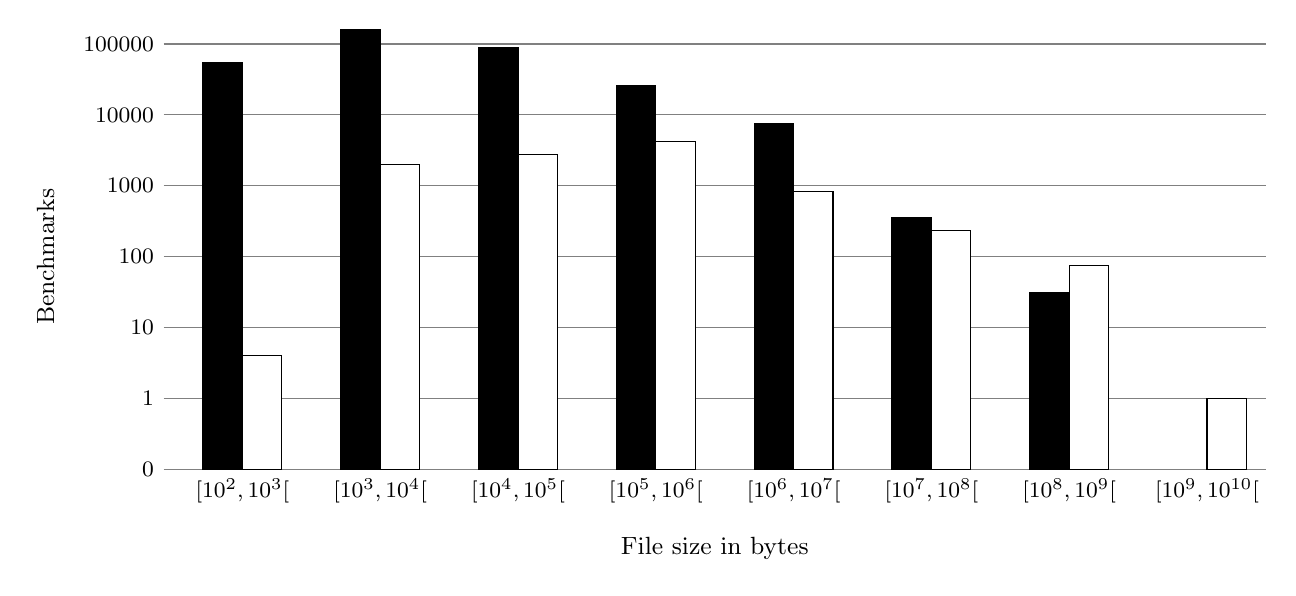
\begin{tikzpicture}
    \draw [gray] (0,0) -- (14,0);
    \draw [gray] (0,.9) -- (14,.9);
    \draw [gray] (0,1.8) -- (14,1.8);
    \draw [gray] (0,2.7) -- (14,2.7);
    \draw [gray] (0,3.6) -- (14,3.6);
    \draw [gray] (0,4.5) -- (14,4.5);
    \draw [gray] (0,5.4) -- (14,5.4);

    \node [left] at (0,0) {\footnotesize 0};
    \node [left] at (0,.9) {\footnotesize 1};
    \node [left] at (0,1.8) {\footnotesize 10};
    \node [left] at (0,2.7) {\footnotesize 100};
    \node [left] at (0,3.6) {\footnotesize 1000};
    \node [left] at (0,4.5) {\footnotesize 10000};
    \node [left] at (0,5.4) {\footnotesize 100000};

    \node [rotate=90] at (-1.5,2.7) {\small Benchmarks};

    \draw [fill=black] (0.5,0) rectangle (1,5.1629791157); % 54531
    \draw [fill=black] (2.25,0) rectangle (2.75,5.5836542368); % 159978
    \draw [fill=black] (4,0) rectangle (4.5,5.350394013); % 88081
    \draw [fill=black] (5.75,0) rectangle (6.25,4.8786283826); % 26345
    \draw [fill=black] (7.5,0) rectangle (8,4.3889077926); % 7526
    \draw [fill=black] (9.25,0) rectangle (9.75,3.1918883971); % 352
    \draw [fill=black] (11,0) rectangle (11.5,2.2422255245); % 31
    %\draw [fill=black] (12.75,0) rectangle (13.25,0); % 0

    \draw [fill=white] (1,0) rectangle (1.5,1.4418539922); % 4
    \draw [fill=white] (2.75,0) rectangle (3.25,3.8742353084); % 2017
    \draw [fill=white] (4.5,0) rectangle (5,3.9968181739); % 2760
    \draw [fill=white] (6.25,0) rectangle (6.75,4.1649057286); % 4243
    \draw [fill=white] (8,0) rectangle (8.5,3.5266990775); % 829
    \draw [fill=white] (9.75,0) rectangle (10.25,3.0372735114); % 237 
    \draw [fill=white] (11.5,0) rectangle (12,2.5927322331); % 76
    \draw [fill=white] (13.25,0) rectangle (13.75,0.9); % 1
    
    \node [below] at (1,0) {\footnotesize $[10^2, 10^3[$};
    \node [below] at (2.75,0) {\footnotesize $[10^3, 10^4[$};
    \node [below] at (4.5,0) {\footnotesize $[10^4, 10^5[$};
    \node [below] at (6.25,0) {\footnotesize $[10^5, 10^6[$};
    \node [below] at (8,0) {\footnotesize $[10^6, 10^7[$};
    \node [below] at (9.75,0) {\footnotesize $[10^7, 10^8[$};
    \node [below] at (11.5,0) {\footnotesize $[10^8, 10^9[$};
    \node [below] at (13.25,0) {\footnotesize $[10^9, 10^{10}[$};

    \node [] at (7,-1) {\small File size in bytes};
  \end{tikzpicture}}
  \caption{Distribution of SMT-LIB benchmarks by file size (2018), for
    non-incremental~($\blacksquare$) and incremental~($\square$)
    benchmarks.}
  \label{fig:benchmark-sizes}
\end{figure}

Benchmarks in the SMT Library are annotated with additional
information, such as the source of the benchmark and its status (i.e.,
whether the benchmark is satisfiable or unsatisfiable) if this is
known.  (For incremental benchmarks, each {\tt check-sat} command has
a separate status annotation.)  To prevent solvers from simply looking
up the benchmark's status in the SMT Library, benchmarks in the
competition are lightly scrambled before they are presented to
solvers~\cite{DBLP:conf/cade/Weber16}.

%%%%%%%%%%%%%%%%%%%%%%%%%%%%%%%%%%%%%%%%%%%%%%%%%%%%%%%%%%%%%%%%%%%%%%%%%%%%%%%%

\section{Competition Divisions and Benchmarks}
\label{sec:benchmarks}

The SMT Competition consists of several tracks.  The \emph{main
  track}, which has been a staple of the competition since its
inception in 2005, features non-incremental benchmarks.  The
\emph{application track}, which has been part of the competition since
2011~\cite{TODO}, features incremental benchmarks.  These benchmarks
are passed to each solver one command at a time by a trace executor,
which waits for the solver's response before passing the next
benchmark command (to prevent look-ahead behavior).  The
\emph{unsat-core track} uses main-track benchmarks that are known to
be unsatisfiable, and solvers are evaluated on their ability to find
small unsatisfiable cores (i.e., a small but still unsatisfiable
subset of the benchmark's assertions).  The unsat-core track had first
been part of the competition in 2012~\cite{TODO}, but was then
discontinued partly because of the competition's move to StarExec and
lacking tool support.  It was re-introduced as an experimental track
in 2016, and has been a regular competition track again since~2017.

Each track is further split into (logic) \emph{divisions}, where each
division corresponds to a logic from the SMT Library.
Table~\ref{table:divisions} shows the number of divisions in each
track since~2015.  Participants can choose which tracks and divisions
they want to enter, and competition results are reported separately
for each track and division.  Thus, competing solvers need not support
all logics, and may or may not support features such as incrementality
or unsat-core generation.

There are slightly fewer divisions than logics in the SMT Library
(Table~\ref{table:smtlib}) because not every logic contains benchmarks
eligible for the competition.  Some benchmarks typically have to be
excluded for syntactic reasons: in 2015 and 2016, 11,966 benchmarks
were excluded because they contained partial or underspecified
operations (e.g., bit-vector division) whose precise semantics were
being debated at the time.  Additionally in 2016, one benchmark was
excluded because it contained incorrect status information.  In 2017,
1,104 benchmarks were excluded because their logic had been classified
incorrectly, and 8 benchmarks were excluded because of incorrect or
missing status information.  Moreover, divisions containing datatypes
({DT})---which were new in~2017---were excluded from the unsat-core
track because of lacking tool support.  In 2018, 3,603 benchmarks were
excluded because they contained named terms (a feature of the SMT-LIB
language that is not permitted in competition benchmarks), and 5
benchmarks were excluded because of missing status information.

\begin{table}
  \caption{Number of divisions in each competition track}
  \label{table:divisions}
  \centering
  \begin{tabular}{|l|r|r|r|r|}
    \hline
    & \multicolumn{1}{c|}{2015} & \multicolumn{1}{c|}{2016} & \multicolumn{1}{c|}{2017} & \multicolumn{1}{c|}{2018} \\
    \hline
    Main track        &  40 & 40 & 49 & 50 \\
    Application track &  14 & 14 & 16 & 21 \\
    Unsat-core track  &  -- & 40 & 41 & 44 \\
    \hline
  \end{tabular}
\end{table}

SMT Competitions until~2014 employed a pseudo-random selection process
to further cull the number of benchmarks used in the competition.
However, a 2013 evaluation of SMT-COMP and SMT-LIB found that this
``significantly lessens the ability of a competition to determine
`best' solvers.''~\cite{CSW15} rTogether with the increased
computational resources available to the competition since its move to
StarExec, this prompted a paradigm shift.  Since 2015, the competition
is evaluating all solvers on all eligible benchmarks. \TODO: benchmark
weights

Another paradigm shift concerns the treatment of benchmarks with
unknown status.  Because of the difficulty to judge solver responses
for such benchmarks, SMT Competitions until 2015 only used benchmarks
whose status was known (i.e., that had been solved previously by
existing SMT solvers).  In 2015, 30,717 non-incremental benchmarks
from the SMT Library were not used for the competition because their
status was unknown.  However, this approach was criticized for
favoring imitation of existing solvers over true innovation.  In~2016,
the SMT Library contained 29,724 non-incremental benchmarks with
unknown status; solver performance on these was evaluated but reported
separately.  Since 2017, all non-incremental benchmarks are eligible
for the competition's main track regardless of status, and they
directly affect the competition results.  Solver responses for such
benchmarks are assumed to be correct, unless there is a disagreement
between two or more (otherwise sound) solvers.  Benchmarks with
disagreements are removed from the competition results (see
Section~\ref{sec:results-disagreements} for further discussion).

For incremental benchmarks, the situation is different: an incremental
benchmark is ineligible for the application track if its first {\tt
  check-sat} command has unknown status.  Otherwise, the prefix of the
benchmark that only contains {\tt check-sat} commands with known
status is eligible.  The main reason for this difference is that the
competition tools for the application track (in particular, the trace
executor) have not been adapted yet to support {\tt check-sat}
commands with unknown status.

Tables~\ref{table:benchmarks-main-track}--\ref{table:benchmarks-unsat-core-track}
show the number of benchmarks that were used in each competition track
and division since~2015.  A dash indicates that no eligible benchmarks
were available, and hence the corresponding SMT-LIB logic was not
actually a competition division in that track and year.  The size of
divisions varies widely, from just one benchmark in ABVFP to~72,705
benchmarks in QF\_SLIA.

\begin{table}
  \caption{Number of benchmarks used in the main track (by division)}
  \label{table:benchmarks-main-track}
  \centering
  \scalebox{.9}[.82]{\begin{tabular}{|l|r|r|r|r|}
    \hline
    Division & \multicolumn{1}{c|}{2015} & \multicolumn{1}{c|}{2016} & \multicolumn{1}{c|}{2017} & \multicolumn{1}{c|}{2018} \\
    \hline
    ABVFP      &     -- &     -- &      1 &     1 \\
    ALIA       &     42 &     42 &     42 &    42 \\
    AUFBVDTLIA &     -- &     -- &   1709 &  1709 \\
    AUFDTLIA   &     -- &     -- &    728 &   728 \\
    AUFLIA     &      4 &      4 &      4 &     4 \\
    AUFLIRA    &  19849 &  19849 &  20011 & 20011 \\
    AUFNIRA    &   1050 &   1050 &   1480 &  1480 \\
    BV         &     85 &     85 &   5151 &  5751 \\
    BVFP       &     -- &     -- &     24 &    24 \\
    FP         &     -- &     -- &     61 &    61 \\
    LIA        &    201 &    201 &    388 &   388 \\
    LRA        &    339 &    339 &   2419 &  2419 \\
    NIA        &      9 &      9 &     14 &    14 \\
    NRA        &   3788 &   3788 &   3811 &  3813 \\
    QF\_ABV    &  14720 &  14720 &  15061 & 15066 \\
    QF\_ABVFP  &     -- &     -- &  18129 & 18129 \\
    QF\_ALIA   &    134 &    139 &    139 &   139 \\
    QF\_ANIA   &      6 &      8 &      8 &     8 \\
    QF\_AUFBV  &     37 &     37 &     31 &    31 \\
    QF\_AUFLIA &   1009 &   1009 &   1009 &  1009 \\
    QF\_AUFNIA &     21 &     21 &     17 &    17 \\
    QF\_AX     &    551 &    551 &    551 &   551 \\
    QF\_BV     &  26414 &  26414 &  40043 & 40102 \\
    QF\_BVFP   &      7 &      7 &  17215 & 17215 \\
    QF\_DT     &     -- &     -- &   8000 &  8000 \\
    QF\_FP     &  34413 &  34413 &  40302 & 40300 \\
    QF\_IDL    &   2094 &   2094 &   2193 &  2193 \\
    QF\_LIA    &   5839 &   5839 &   6141 &  6947 \\
    QF\_LIRA   &      6 &      6 &      7 &     7 \\
    QF\_LRA    &   1626 &   1626 &   1649 &  1649 \\
    QF\_NIA    &   8475 &   8593 &  23876 & 23876 \\
    QF\_NIRA   &      2 &      2 &      3 &     3 \\
    QF\_NRA    &  10184 &  10245 &  11354 & 11489 \\
    QF\_RDL    &    220 &    220 &    255 &   255 \\
    QF\_SLIA   &     -- &     -- &     -- & 72705 \\
    QF\_UF     &   6649 &   6649 &   6650 &  7423 \\
    QF\_UFBV   &     31 &     31 &     31 &  1224 \\
    QF\_UFIDL  &    441 &    441 &    428 &   428 \\
    QF\_UFLIA  &    598 &    598 &    583 &   583 \\
    QF\_UFLRA  &   1627 &   1627 &   1284 &  1284 \\
    QF\_UFNIA  &      7 &      7 &      7 &     7 \\
    QF\_UFNRA  &     34 &     34 &     36 &    36 \\
    UF         &   2839 &   2839 &   7562 &  7562 \\
    UFBV       &     71 &     71 &    200 &   200 \\
    UFDT       &     -- &     -- &   4535 &  4527 \\
    UFDTLIA    &     -- &     -- &    303 &   303 \\
    UFIDL      &     68 &     68 &     68 &    68 \\
    UFLIA      &   8404 &   8404 &  10137 & 10137 \\
    UFLRA      &     25 &     25 &     15 &    15 \\
    UFNIA      &   2319 &   2319 &   3308 &  3308 \\
    \hline
    Total      & 154238 & 154424 & 256973 & 333241 \\
    \hline
  \end{tabular}}
\end{table}

\begin{table}
  \caption{Number of benchmarks used in the application track (by
    division)}
  \label{table:benchmarks-application-track}
  \centering
  \begin{tabular}{|l|r|r|r|r|}
    \hline
    Division & \multicolumn{1}{c|}{2015} & \multicolumn{1}{c|}{2016} & \multicolumn{1}{c|}{2017} & \multicolumn{1}{c|}{2018} \\
    \hline
    ALIA       &   24 &   24 &   24 &   24 \\
    ANIA       &    3 &    3 &    3 &    3 \\
    AUFNIRA    &   -- &   -- &   -- &  117 \\
    BV         &   -- &   -- &   -- &   17 \\
    LIA        &    6 &    6 &    6 &    6 \\
    QF\_ABV    &   -- &   -- &   -- &   15 \\
    QF\_ALIA   &   44 &   44 &   44 &   44 \\
    QF\_ANIA   &    5 &    5 &    5 &    5 \\
    QF\_AUFBV  &   -- &   -- &   -- &   10 \\
    QF\_AUFLIA &   72 &   72 &   72 &   72 \\
    QF\_BV     &   18 &   18 &   18 &  815 \\
    QF\_BVFP   &   -- &   -- &    2 &    2 \\
    QF\_FP     &   -- &   -- &    2 &    2 \\
    QF\_LIA    &   65 &   69 &   68 &   69 \\
    QF\_LRA    &   10 &   10 &   10 &   10 \\
    QF\_NIA    &   10 &   10 &   10 &   10 \\
    QF\_UFBV   &   -- &   -- &   -- & 2327 \\
    QF\_UFLIA  &  905 &  905 &  780 &  780 \\
    QF\_UFLRA  & 3331 & 3331 & 3056 & 3058 \\
    QF\_UFNIA  &    1 &    1 &    1 &    1 \\
    UFLRA      & 5358 & 5358 & 1870 & 1870 \\
    \hline
    Total      & 9852 & 9856 & 5971 & 9257 \\
    \hline
  \end{tabular}
\end{table}

\begin{table}
  \caption{Number of benchmarks used in the unsat-core track (by
    division)}
  \label{table:benchmarks-unsat-core-track}
  \centering
  \scalebox{1}[.93]{\begin{tabular}{|l|r|r|r|}
    \hline
    Division & \multicolumn{1}{c|}{2016} & \multicolumn{1}{c|}{2017} & \multicolumn{1}{c|}{2018} \\
    \hline
    ALIA       &     41 &     41 &     41 \\
    AUFBVDTLIA &     -- &     -- &     25 \\
    AUFLIA     &      3 &      3 &      3 \\
    AUFLIRA    &  19749 &  19771 &  19771 \\
    AUFNIRA    &   1046 &   1050 &   1053 \\
    BV         &     56 &     94 &   4937 \\
    LIA        &    191 &    233 &    233 \\
    LRA        &    319 &   1106 &   1539 \\
    NIA        &      3 &      4 &      4 \\
    NRA        &   3788 &   3801 &   3801 \\
    QF\_ABV    &   4644 &   4673 &   4677 \\
    QF\_ABVFP  &     -- &   3934 &   3934 \\
    QF\_ALIA   &     80 &     80 &     80 \\
    QF\_ANIA   &      8 &      8 &      8 \\
    QF\_AUFBV  &     31 &     25 &     25 \\
    QF\_AUFLIA &    516 &    516 &    516 \\
    QF\_AUFNIA &     15 &     12 &     12 \\
    QF\_AX     &    279 &    279 &    279 \\
    QF\_BV     &  17172 &  23732 &  25700 \\
    QF\_BVFP   &      6 &   3174 &   3174 \\
    QF\_DT     &     -- &     -- &   4422 \\
    QF\_FP     &  17213 &  20028 &  20026 \\
    QF\_IDL    &    816 &    816 &    816 \\
    QF\_LIA    &   2840 &   2844 &   3019 \\
    QF\_LIRA   &      5 &      5 &      5 \\
    QF\_LRA    &    633 &    671 &    683 \\
    QF\_NIA    &    316 &   3130 &   4842 \\
    QF\_NIRA   &      2 &      2 &      2 \\
    QF\_NRA    &   4948 &   5296 &   5357 \\
    QF\_RDL    &    113 &    113 &    113 \\
    QF\_UF     &   4100 &   4101 &   4330 \\
    QF\_UFBV   &     31 &     31 &    575 \\
    QF\_UFIDL  &    335 &    322 &    322 \\
    QF\_UFLIA  &    195 &    183 &    183 \\
    QF\_UFLRA  &    853 &    511 &    511 \\
    QF\_UFNIA  &      7 &      7 &      7 \\
    QF\_UFNRA  &     18 &     11 &     11 \\
    UF         &   2039 &   3316 &   3442 \\
    UFBV       &     53 &     97 &     97 \\
    UFDT       &     -- &     -- &   1863 \\
    UFIDL      &     62 &     57 &     57 \\
    UFLIA      &   8377 &   7714 &   7743 \\
    UFLRA      &     20 &     10 &     10 \\
    UFNIA      &   2318 &   2432 &   2457 \\
    \hline
    Total      &  93241 & 114233 & 130705 \\
    \hline
  \end{tabular}}
\end{table}

%%%%%%%%%%%%%%%%%%%%%%%%%%%%%%%%%%%%%%%%%%%%%%%%%%%%%%%%%%%%%%%%%%%%%%%%%%%%%%%%

\section{Infrastructure}
\label{sec:starexec}

Since 2014 (and previously for the evaluation in 2013~\cite{CSW15}),
the computational workload of the competition is being run on
StarExec, a ``cross-community infrastructure for logic
solving''~\cite{DBLP:conf/cade/StumpST14} developed at the University
of Iowa and supported by the National Science Foundation.  Each
machine in the StarExec cluster is equipped with two E5-2609 Intel
Xeon processors (10~MiB Cache, 2.4~GHz).  This hardware configuration
has been unchanged since~2013.  Up to two solvers are run
simultaneously on each machine: one solver on each processor, with
four cores available.  Memory usage is limited to~60~GiB per solver.

On the software side, the cluster is running Red Hat Enterprise Linux
Workstation.  The~2015 competition was running on release~6.3
(Santiago, kernel 2.6.32-431).  This was updated to~7.2 (Maipo, kernel
3.10.0-327) before the~2016 competition, and the kernel was further
updated to~3.10.0-514 before the~2017 competition.  The platform
emphasizes stability over bleeding edge technology.  This has on
occasion caused problems with solver binaries that had been compiled
on other Linux distributions and linked against library versions not
(yet) available on the cluster.  Usually, such problems are easily
solved by building the solver on StarExec instead.  The StarExec
developers have made a virtual machine image available to facilitate
this and similar tasks.

Interaction with StarExec is mostly via its web interface,
\url{https://www.starexec.org}.  The interface allows registered users
to upload and share benchmarks and solvers, to create and manage jobs
that apply selected solvers to a selection of benchmarks, and to view
and download job results.  Other features, such as pre-processing of
benchmarks (e.g., for scrambling) and post-processing of solver
output, are also supported.

Jobs consist of individual \emph{job pairs}.  Each job pair
corresponds to a specific solver-benchmark combination.
Figure~\ref{fig:job-pairs} shows the total number of job pairs for the
SMT Competition from~2015 to~2018.  Over this period, the number has
grown by~72\,\%, from~1,028,615 job pairs in~2015 to~1,776,062 job
pairs in~2018.  (This is the number of unique solver-benchmark
combinations that were part of the competition.  The number of job
pairs that were actually run is even higher: test jobs and job pairs
that had to be re-run, e.g., because of issues with the StarExec
infrastructure, are not included.)  For comparison, the~2014
competition only ran~339,714 job pairs~\cite{CDW14}.

Also shown in Figure~\ref{fig:job-pairs} is the total wall-clock time
(summed over all job pairs) for the competition.  This has more than
doubled, from 3.5~years in~2015 to 7.6~years in~2018.  (These are
solver run-times only.  Time that the cluster spent on pre- and
post-processing of benchmarks and solver output or on other auxiliary
tasks is not included.)  The increase in~2016 is largely due to the
inclusion of non-incremental benchmarks with unknown status; these
were evaluated with a wall-clock time limit of 10~minutes.  In~2017,
when these benchmarks had become eligible for the main track,
main-track job pairs were first run with a time limit of 10~minutes;
when it became apparent to the organizers that there were sufficient
resources to increase this limit, job pairs that had timed out were
re-run with a time limit of 20~minutes.  Table~\ref{table:time-limits}
shows the wall-clock time limits that were imposed for each track and
year.

\begin{table}
  \caption{Wall-clock time limits}
  \label{table:time-limits}
  \centering
  \begin{tabular}{|l|r|r|r|r|}
    \hline
    & \multicolumn{1}{c|}{2015} & \multicolumn{1}{c|}{2016} & \multicolumn{1}{c|}{2017} & \multicolumn{1}{c|}{2018} \\
    \hline
    Main track        & 40~min & 40~min & 20~min & 20~min \\
    Application track & 40~min & 40~min & 40~min & 40~min \\
    Unsat-core track  &     -- & 40~min & 40~min & 40~min \\
    \hline
  \end{tabular}
\end{table}

StarExec typically reserves between~80 and~150 machines for the SMT
Competition, allowing its workload to be completed within two to three
weeks.  By these measures, the SMT Competition has become not only one
of the heaviest users of StarExec, but also one of the largest
competitions in automated reasoning.

\begin{figure}
  \centering
  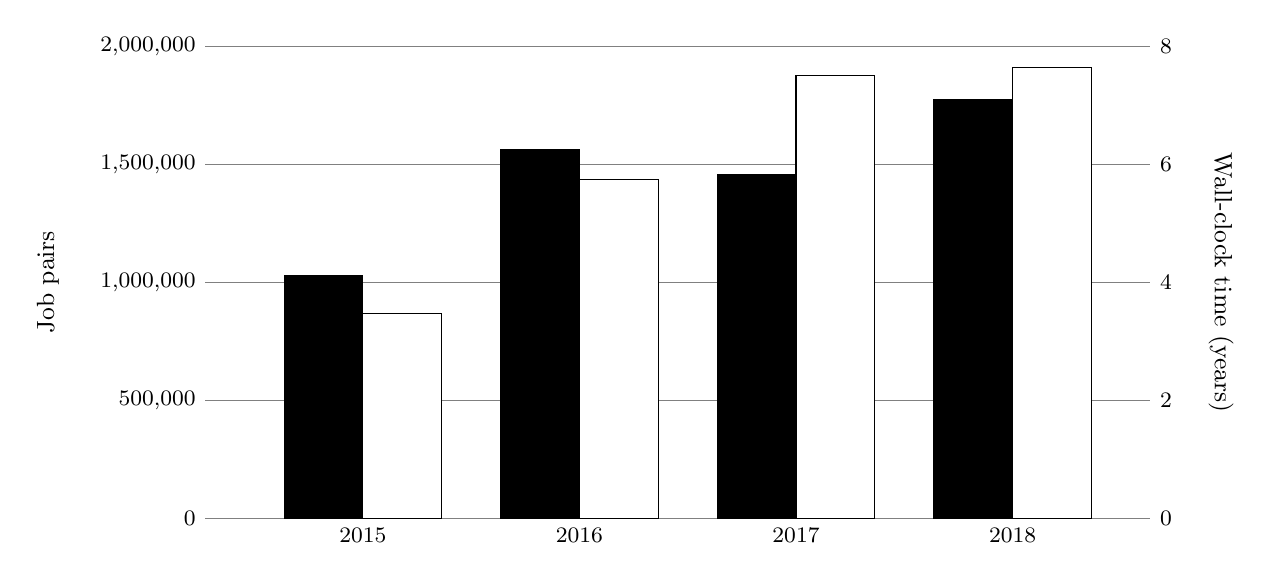
\begin{tikzpicture}
    \draw [gray] (0,0) -- (12,0);
    \draw [gray] (0,1.5) -- (12,1.5);
    \draw [gray] (0,3) -- (12,3);
    \draw [gray] (0,4.5) -- (12,4.5);
    \draw [gray] (0,6) -- (12,6);

    \node [left] at (0,0) {\footnotesize 0};
    \node [left] at (0,1.5) {\footnotesize 500,000};
    \node [left] at (0,3) {\footnotesize 1,000,000};
    \node [left] at (0,4.5) {\footnotesize 1,500,000};
    \node [left] at (0,6) {\footnotesize 2,000,000};

    \node [rotate=90] at (-2,3) {\small Job pairs};

    \node [right] at (12,0) {\footnotesize 0};
    \node [right] at (12,1.5) {\footnotesize 2};
    \node [right] at (12,3) {\footnotesize 4};
    \node [right] at (12,4.5) {\footnotesize 6};
    \node [right] at (12,6) {\footnotesize 8};

    \node [rotate=-90] at (12.9,3) {\small Wall-clock time (years)};

    \draw [fill=black] (1,0) rectangle (2,3.085845); % 1,028,615
    \draw [fill=black] (3.75,0) rectangle (4.75,4.687632); % 1,562,544
    \draw [fill=black] (6.5,0) rectangle (7.5,4.366839); % 1,455,613
    \draw [fill=black] (9.25,0) rectangle (10.25,5.328186); % 1,776,062

    \draw [fill=white] (2,0) rectangle (3,2.6088709094); % 3,4784945459
    \draw [fill=white] (4.75,0) rectangle (5.75,4.3030490392); % 5,7373987189
    \draw [fill=white] (7.5,0) rectangle (8.5,5.6286127759); % 7,5048170345
    \draw [fill=white] (10.25,0) rectangle (11.25,5.7280186691); % 7,6373582255

    \node [below] at (2,0) {\footnotesize 2015};
    \node [below] at (4.75,0) {\footnotesize 2016};
    \node [below] at (7.5,0) {\footnotesize 2017};
    \node [below] at (10.25,0) {\footnotesize 2018};
  \end{tikzpicture}
  \caption{Number of job pairs ($\blacksquare$) and total wall-clock time ($\square$).}
  \label{fig:job-pairs}
\end{figure}

The StarExec infrastructure has been vitally important in allowing the
competition to grow to its current size.  The competition organizers
have given the StarExec developers comprehensive feedback, and filed
dozens of feature requests and bug reports since~2013.  The
infrastructure has become increasingly stable; serious issues are now
rare.  When they did surface during an ongoing competition, they
received a swift response by the StarExec team (under the lead of
Aaron Stump).  This has been critical to the success of the
competition on more than one occasion.

%%%%%%%%%%%%%%%%%%%%%%%%%%%%%%%%%%%%%%%%%%%%%%%%%%%%%%%%%%%%%%%%%%%%%%%%%%%%%%%%

\section{Participants}
\label{sec:participants}

Participants must upload their solvers to StarExec to enter them into
the competition, and additionally submit information about each
competing solver---such as the tracks and divisions into which the
solver is being entered---to the competition organizers.  Until 2016,
this information was collected by email.  Since 2017, a web form is
being used for this purpose.  This has greatly reduced the number of
incomplete or ambiguous submissions.

Table~\ref{table:participants} lists the solvers that participated
between~2015 and~2018, together with their submitter(s) and
institutional affiliations (which may have changed over time).  Note
that most solvers were developed by a group of people; the table does
not list all contributors but only submitters.
%
Participants are also encouraged to submit a short system description
of their solver, including a list of its authors and an explanation of
the SMT solving approach used.  System descriptions are published on
the SMT-COMP website~\cite{smtcomp-web}.  They were submitted for
about 60\,\% of all solver versions since 2015.

\begin{table}
  \caption{Participants (2015--2018)}
  \label{table:participants}
  \centering
  \begin{tabular}{|l|p{13cm}|} %TODO: fix width
    \hline
    Solver & Submitters (Affiliations)\\
    \hline
    ABC [\TODO]       & Valeriy Balabanov
                        (Mentor Graphics)\\
    Alt-Ergo          & Albin Coquereau
                        (CNRS and University of Paris-Sud)\\
    AProVE            & Carsten Fuhs
                        (University College London; Birkbeck, University of London)\\
    Boolector         & Mathias Preiner
                        (Johannes Kepler University)\\
    COLIBRI           & Fran\c{c}ois Bobot
                        (French Alternative Energies and Atomic Energy Commission)\\
    Ctrl-Ergo         & Mohamed Iguernlala
                        (CNRS and University of Paris-Sud)\\
    CVC3              & Kshitij Bansal
                        (New York University)\\
    CVC4              & Kshitij Bansal, Clark Barrett, Andres N\"otzli, Duligur Ibeling
                        (New York University; Stanford University)\\
    MapleSTP          & Jimmy Liang
                        (University of Waterloo)\\
    MinkeyRink        & Trevor Hansen
                        (University of Melbourne)\\
    OpenSMT2          & Matteo Marescotti, Antti Hyv\"arinen
                        (University of Lugano)\\
    ProB              & Sebastian Krings
                        (University of D\"usseldorf)\\
    Q3B               & Martin Jon\'a\v{s}
                        (Masaryk University)\\
    raSAT             & Tung Vu Xuan
                        (Japan Advanced Institute of Science and Technology)\\
    Redlog            & Haniel Barbosa
                        (Inria Nancy)\\
    SMT-RAT           & Florian Corzilius, Gereon Kremer
                        (RWTH Aachen University)\\
    SMTInterpol       & J\"urgen Christ
                        (University of Freiburg)\\
    SPASS-SATT        & Martin Bromberger
                        (Max Planck Institute for Informatics)\\
    STP               & Mate Soos, Trevor Hansen, Norbert Manthey
                        (National University of Singapore; University of Melbourne; Amazon Web Services)\\
    toysmt            & Masahiro Sakai
                        (Toshiba Corporation)\\
    Vampire           & Giles Reger
                        (University of Manchester)\\
    veriT             & David D\'eharbe, Haniel Barbosa, Hans-J\"org Schurr
                        (Federal University of Rio Grande do Norte; Inria Nancy)\\
    XSat              & Martin Velez
                        (University of California, Davis)\\
    Yices2            & Bruno Dutertre, Dejan Jovanovi\'c
                        (SRI International)\\
    Z3                & Christoph Wintersteiger, Aleksandar Zelji\'c
                        (Microsoft Research; Uppsala University)\\
    \hline
  \end{tabular}
\end{table}

Many of these solvers were submitted in multiple years.  Additionally,
to promote a wide comparison between tools, developers are allowed to
submit multiple versions of a solver, e.g., for different competition
tracks or with differently tuned internal components.
Table~\ref{table:participants-history} shows in more detail how many
versions of each solver were submitted in each year.

\begin{table}
  \caption{Number of versions submitted for each solver (by year).
    Numbers in square brackets indicate solver versions that were
    participating hors concours.}
  \label{table:participants-history}
  \centering
  \begin{tabular}{|l|r@{\,\,}r|r@{\,\,}r|r@{\,\,}r|r@{\,\,}r|}
    \hline
    Solver & \multicolumn{2}{c|}{2015} & \multicolumn{2}{c|}{2016} & \multicolumn{2}{c|}{2017} & \multicolumn{2}{c|}{2018} \\
    \hline
    ABC               &    &      &  2 &      &    &      &    &      \\
    Alt-Ergo          &    &      &    &      &    &      &  1 &      \\
    AProVE            &  1 &      &  1 &      &  1 &      &  1 &      \\
    Boolector         &  3 & [+1] &  2 &      &  2 &      &  2 &      \\
    COLIBRI           &    &      &    &      &  1 &      &  1 &      \\
    Ctrl-Ergo         &    &      &    &      &    &      &  1 &      \\
    CVC3              &  2 &      &    &      &    &      &    &      \\
    CVC4              &  4 &      &  1 & [+1] &  3 &      &  3 & [+1] \\
    MapleSTP          &    &      &  4 &      &    &      &    &      \\
    {[}MathSAT{]}     &    & [+2] &    & [+3] &    & [+3] &    & [+3] \\
    MinkeyRink        &    &      &  1 &      &  1 &      &  2 &      \\
    OpenSMT2          &  2 &      &  1 &      &  1 &      &    & [+1] \\
    ProB              &    &      &  1 &      &    &      &    &      \\
    Q3B               &    &      &  1 &      &  1 &      &  1 &      \\
    raSAT             &  1 &      &  2 &      &    &      &    &      \\
    Redlog            &    &      &    &      &  1 &      &    &      \\
    SMT-RAT           &  2 &      &  1 &      &  1 &      &  2 &      \\
    SMTInterpol       &  1 &      &  1 &      &  1 &      &  1 &      \\
    SPASS-SATT        &    &      &    &      &    &      &  1 &      \\
    STP               &  4 &      &  8 &      &  2 &      &  3 &      \\
    toysmt            &    &      &  1 &      &    &      &    &      \\
    Vampire           &    &      &  2 &      &  1 &      &  1 &      \\
    veriT             &  1 &      &  1 &      &  3 &      &  2 &      \\
    XSat              &    &      &    &      &  1 &      &    &      \\
    Yices2            &  3 &      &  2 &      &  2 &      &  3 &      \\
    Z3                &  2 & [+1] &    & [+1] &    & [+1] &    & [+1] \\
    \hline
    Total             & 26 & [+4] & 32 & [+5] & 22 & [+4] & 25 & [+6] \\
    \hline
  \end{tabular}
\end{table}

In addition to the solvers that were submitted to the competition by
their respective developers, the organizers included the most recent
stable versions of MathSAT and Z3 for comparison purposes.  Both
solvers are strong tools, but---except for two experimental versions
of Z3 in 2015---their development teams chose not to prepare
competition versions.  These solvers were therefore participating hors
concours.  Moreover, in 2015 a bug was discovered in the application
track version of Boolector and a fixed version was submitted after the
deadline; in 2016, the CVC4 team did not enter their solver into the
application track; and in 2018, an experimental version of CVC4 as
well as the OpenSMT2 solver were submitted after the deadline.  These
solvers were also participating hors concours.  In result tables, they
are listed with their name in square brackets (e.g., [MathSAT]).

Table~\ref{table:participation-by-track} summarizes these figures and
shows how many solver versions were submitted to each track of the
competition.  Note that solver versions may be entered into multiple
tracks.  Therefore, the total number of solver versions for each year
is typically less than the sum over all tracks.

By number of solver versions submitted, the competitions in 2015--2018
were the four largest in the history of SMT-COMP.  On average, 26
solver versions were submitted each year since 2015.  In contrast, the
competitions from 2005--2014 only received an average of 12
submissions~\cite{CDW14}.

\begin{table}
  \caption{Participation by track and year.  Numbers in square
    brackets indicate solver versions that were participating hors
    concours.}
  \label{table:participation-by-track}
  \centering
  \begin{tabular}{|l|r@{\,\,}r|r@{\,\,}r|r@{\,\,}r|r@{\,\,}r|}
    \hline
                      & \multicolumn{2}{c|}{2015} & \multicolumn{2}{c|}{2016} & \multicolumn{2}{c|}{2017} & \multicolumn{2}{c|}{2018} \\
    \hline
    Main track        & 21 &                [+2] & 25 & [+2] & 19 & [+2] & 20 & [+4] \\
    Application track & 10 &                [+3] &  8 & [+3] &  4 & [+2] &  4 & [+2] \\
    Unsat-core track  & \multicolumn{2}{c|}{---} &  1 & [+4] &  2 & [+2] &  3 & [+2] \\
    \hline
    Total             & 26 &                [+4] & 32 & [+5] & 22 & [+4] & 25 & [+6] \\
    \hline
  \end{tabular}
\end{table}

%%%%%%%%%%%%%%%%%%%%%%%%%%%%%%%%%%%%%%%%%%%%%%%%%%%%%%%%%%%%%%%%%%%%%%%%%%%%%%%%

\section{Competition Procedure}
\label{sec:procedure}

\TODO: explain those aspects of the procedure that are required to
understand the results (e.g., time limits, scoring)

%%%%%%%%%%%%%%%%%%%%%%%%%%%%%%%%%%%%%%%%%%%%%%%%%%%%%%%%%%%%%%%%%%%%%%%%%%%%%%%%

\section{Results}
\label{sec:results}

%%%%%%%%%%%%%%%%%%%%%%%%%%%%%%%%%%%%%%%%%%%%%%%%%%%%%%%%%%%%%%%%%%%%%%%%%%%%%%%%

\section{FLoC Olympic Games}
\label{sec:floc}

In 2014, the SMT Competition was part of the FLoC Olympic Games.
These gave the competition increased visibility and sponsored three
Kurt G\"odel medals.  After substantial internal debate, the 2014
competition organizers decided to award these to the winner of the
main track's QF\_BV division (which has historically been the logic
with the largest number of solver submissions and job pairs), as well
as to the two best main-track solvers according to a competition-wide
ranking that had been instituted especially for this
purpose~\cite{DBLP:journals/jsat/CokDW14}.  This ranking emphasizes
breadth of solver participation---a solver participating in many
logics need not be the best in any one of them to rank highly.

The competition-wide ranking for the main track was retained and
refined after~2014.  A contentious issue with this ranking has been
the scoring of incorrect solver responses.  In the per-division
rankings, an incorrect response causes a solver to be ranked behind
all correct solvers~\cite{rules18}.  But the competition's main track
consists of many independent divisions.  To balance the strong
interest in correct solvers against the risk of stifling innovation,
the competition-wide ranking was revised in~2017 to use a fixed
numeric penalty for each division with incorrect responses.  The value
of this penalty is currently set so that entering a (possibly buggy)
solver that can solve all benchmarks into a division has a positive
expected score if the probability of a soundness bug in the solver is
below~$20\,\%$.

The 2018 edition of the competition was again part of the FLoC Olympic
Games, which sponsored seven medals.  The competition organizers
awarded these to the following solvers:
\begin{itemize}
\item The best three main-track solvers according to the
  competition-wide ranking (first place: CVC4, second place:
  Yices-2.6.0, third place: SMTInterpol);
\item the solver(s) that won the QF\_BV division in the main track
  (sequential ranking: Boolector, parallel ranking: Minkeyrink-MT);
\item the solver that won the most competitive divisions in the
  application track (Yices-2.6.0);
\item the solver that won the most competitive divisions in the
  unsat-core track (Yices-2.6.0).
\end{itemize}

In comparison to the competition-wide ranking for the main track, the
metric used for the application and unsat-core track---simply counting
the number of competitive divisions that a solver has won---was rather
unsophisticated.  Future editions of the competition should perhaps
refine this to use a ranking scheme that is more similar to the
main-track ranking, by weighing divisions according to their relative
importance, and also by rewarding good performance from solvers other
than division winners.  A difficulty in adapting the main-track
ranking for the other tracks is that each main-track benchmark is
worth one point (before weighing) if solved correctly, while
benchmarks in the application and unsat-core track are worth widely
varying numbers of points.  Moreover, in the unsat-core track, the
size of the smallest unsatisfiable core---and hence the number of
points attainable on any given benchmark---may not be known precisely.

%%%%%%%%%%%%%%%%%%%%%%%%%%%%%%%%%%%%%%%%%%%%%%%%%%%%%%%%%%%%%%%%%%%%%%%%%%%%%%%%

\section{Conclusions}
\label{sec:conclusions}

\TODO

inclusion of check-sat commands with unknown status in the application track

competition-wide rankings for application and unsat-core track

more benchmarks, especially for underrepresented (i.e., small) logics

%%%%%%%%%%%%%%%%%%%%%%%%%%%%%%%%%%%%%%%%%%%%%%%%%%%%%%%%%%%%%%%%%%%%%%%%%%%%%%%%

\bibliographystyle{plainbv}
\bibliography{SMT-COMP}

\end{document}

%%%%%%%%%%%%%%%%%%%%%%%%%%%%%%%%%%%%%%%%%%%%%%%%%%%%%%%%%%%%%%%%%%%%%%%%%%%%%%%%

% Local Variables:
% ispell-local-dictionary: "american"
% mode: LaTeX
% mode: flyspell
% LocalWords: concours hors logics satisfiability SMT Tjark
% End:
